\section{Data Analysis}
The goal of this section is to take a first look a the data in order to understand what it represents, then proceed to an in-depth analysis of said data.

\subsection{Data Description}
Data is contained in four different comma-separated values (csv) files: inputs and output for both training and testing. The very first line of each file correspond to the headers. The following lines contain informations about a given product where each product is identified by a unique code:\\

\textbf{ID} = \textbf{PROC\_TRACEINFO} = It's a unique code given to the product.\\
Example: I-B-XA1207672-190701-00494.
\begin{itemize}
    \item XA1207672 is the reference.  
    \item 190701 is the date: here 01st of July of year 2019.  
    \item 00494 is the unique code given to the product, whatever it happens, the product will have this id number frozen forever.
\end{itemize}

This number is increased by 1 each time we process a new product, every 12 seconds. So for example: I-B-XA1207672-190701-00495 is the next product.\\

Input features are measures (numerical values) collected on different assembly stations with the sensors or devices connected to Programmable Logic Controllers which are storing all of them to keep the full quality traceability. Examples : OP070\_V\_1\_angle\_value, OP120\_Rodage\_I\_value...\\

This is the result value of OP130 (test bench). Value 0 is assigned to OK samples (passed) and value 1 is assigned to KO samples (failed). This is the combined result of multiple electrical, acoustic and vibro-acoustic tests.

\subsection{In-Depth Analysis}

Let us put the testing data aside for now and take a closer look a the training data.\\

The training data consists of 13 measures (inputs features) made during production line on just shy of 35000 products. This measures correpond to various forces, angles, screwing torques... By taking a look at the distribution for each feature (Figure \ref{data_analysis_1}) we can clearly see that every one of them has a different shape.\\

\begin{figure}
    \center
    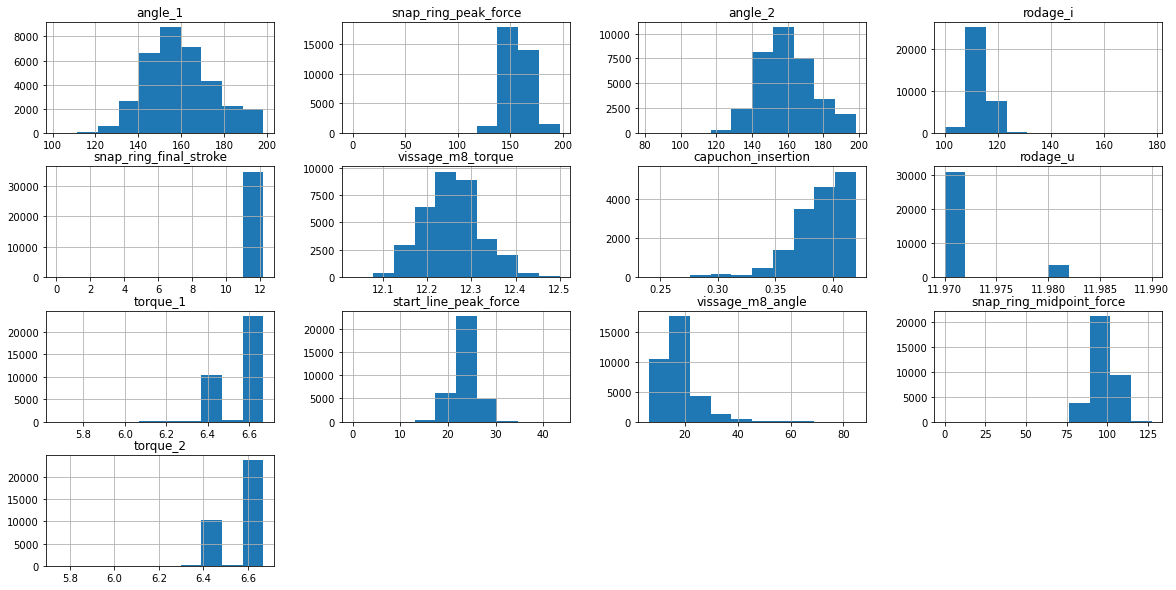
\includegraphics[scale=.38]{img/data_analysis_1.png}
    \caption{Distributions of the input features}
    \label{data_analysis_1}
\end{figure}

An in-depth look at the box-plots (Figure \ref{data_analysis_2}) reveals that there might be some outliers in the dataset.\\

\begin{figure}
    \center
    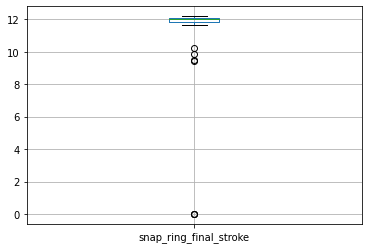
\includegraphics[scale=.5]{img/data_analysis_2.png}
    \caption{Box-plot of the \textit{snap\_ring\_final\_stroke} feature}
    \label{data_analysis_2}
\end{figure}

One feature requires more attention. \textsf{capuchon\_insertion} is the only feature containing missing values. In fact, more than 50\% of the sample population are missing this value.\\

% PCA, relevant?

The training data also contains the result value of the test bench for each product tested on the production line. As expected, there are only a few of defective items. Although this is good for the company, it means that less than 1\% of the training population are defective items. The effectives of the two classes are very unbalanced which could really impact our models.